% !TeX spellcheck = en_US


\chapter{Hardware Design}

This chapter details the hardware design underlying the whisker sensor system.
It covers the whisker mechanical structure, sensor integration, and whisker array assembly.


\section{Magnetically Transduced Whisker Sensor}
The structure of a single whisker sensor is shown in Figure~\ref{fig:whisker_composite}.

\begin{figure}[ht]
    \centering
    \begin{subfigure}[b]{0.31\textwidth}
        \centering
        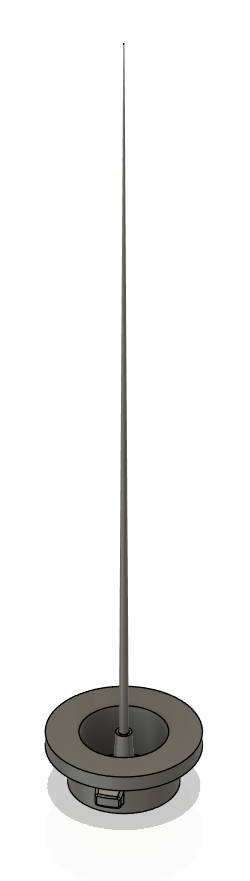
\includegraphics[height=0.2\textheight]{figures/whisker}
        \caption{Whisker mounted on the suspension} \label{fig:whisker}
    \end{subfigure}
    \hspace*{\fill}
    \begin{subfigure}[b]{0.31\textwidth}
        \centering
        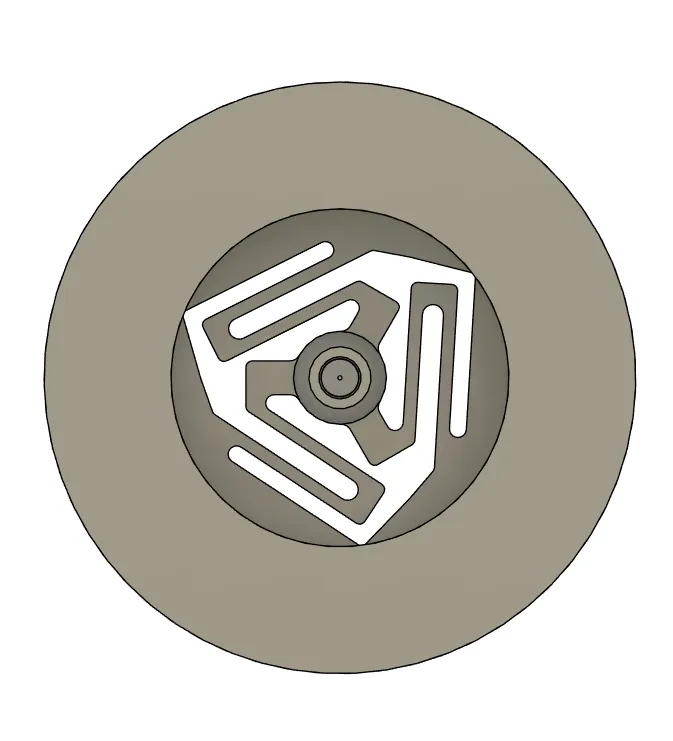
\includegraphics[width=\linewidth]{figures/suspension}
        \caption{Suspension design} \label{fig:suspension}
    \end{subfigure}
    \hspace*{\fill}
    \begin{subfigure}[b]{0.31\textwidth}
        \centering
        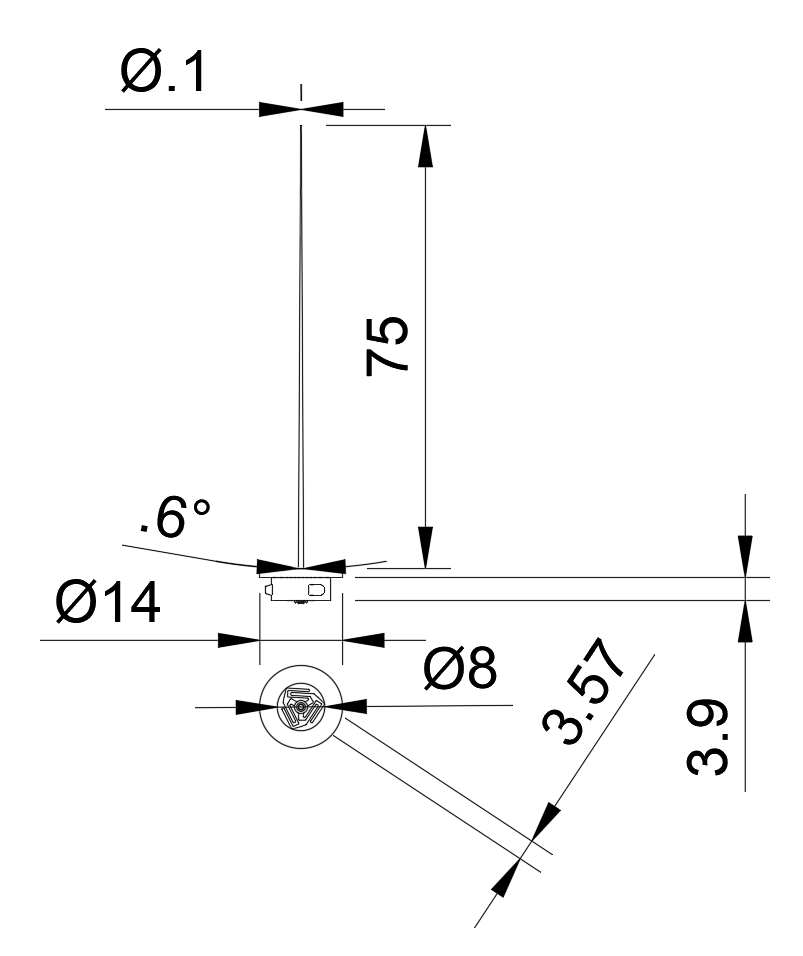
\includegraphics[width=\linewidth]{figures/whisker-dims}
        \caption{Structural dimensions} \label{fig:whisker-dims}
    \end{subfigure}
    \caption{Single whisker sensor.}
    \label{fig:whisker_composite}
\end{figure}

The whisker consists of:
\begin{itemize}
    \item A flexible nitinol wire shaft (\SI{0.25}{\milli\meter} diameter, \SI{75}{\milli\meter} length).
    \item A suspension system fabricated via 3D printing using Polylactic Acid (PLA) filament.
    \item An Adafruit MLX90393 magnetic sensor, configured to measure magnetic flux changes with a resolution of 0.15\,$\mu T$/LSB.
\end{itemize}

The whisker shaft is inserted into and glued to the suspension system.
A neodymium permanent magnet, axially magnetized and aligned with the whisker shaft, is placed directly beneath the suspension.
When the whisker deflects, the magnet rotates, altering the sensed magnetic field.

The suspension is designed to allow slight rotation of the whisker shaft while limiting axial movement.
Three spring-like arms hold the whisker securely in place.


\section{Whisker Platform}

A whisker platform was developed to enable multi-whisker exploration and contour reconstruction.
It consists of a triangular body with a \SI{30}{\degree} nose angle, two side clamps that each hold up to three whiskers, and a mount compatible with the Franka Panda robotic arm gripper.
The platform, depicted in Figure~\ref{fig:platform}, measures \SI{90}{\milli\meter} $\times$ \SI{60}{\milli\meter} $\times$ \SI{35}{\milli\meter} and is 3D printed using PLA filament.
Figure~\ref{fig:whisker_platform} shows the printed and assembled platform, designed to roughly resemble a rat’s shape.

The MLX90393 sensors are secured by side clamps designed with cuts to accommodate 4-pin JST connectors on both sides.
All components are assembled using M2 and M3 screws.

The clamps and suspension bases are designed to allow whiskers to be quickly plugged into place and locked by slight rotation, enabling easy replacement.
No external power supply beyond the JST connector is necessary.

Whiskers are mounted at a \SI{15}{\degree} angle relative to the platform’s mirror plane, slightly pointing forward to enlarge the contact search area.
However, this orientation poses the risk of head-on collisions during tunneling, potentially causing excessive deflection, permanent deformation, or breaking.
Implementing safeguards within the control system to mitigate this is beyond the scope of this thesis.
Thus, in simulations, whiskers are oriented slightly backward to avoid these issues.

\begin{figure}[ht]
    \centering
    \begin{subfigure}[b]{0.45\textwidth}
        \centering
        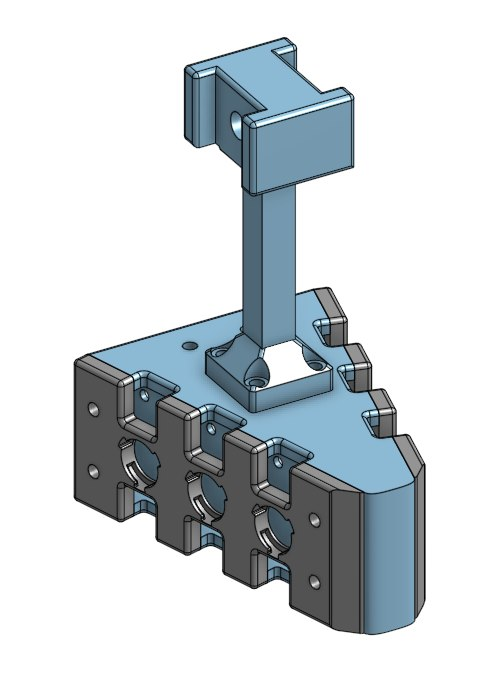
\includegraphics[width=\linewidth]{figures/platform-cad}
        \caption{Platform CAD model.}
    \end{subfigure}
    \hfill
    \begin{subfigure}[b]{0.45\textwidth}
        \centering
        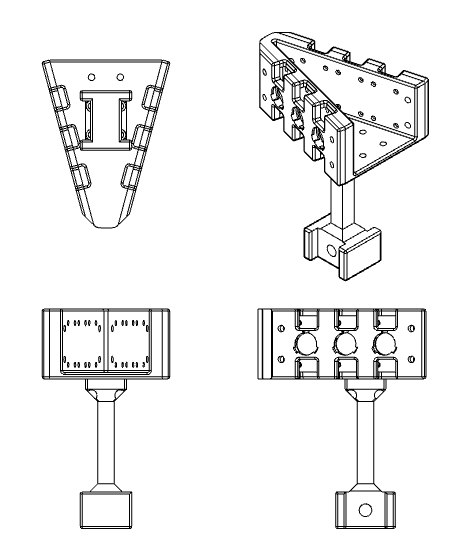
\includegraphics[width=\linewidth]{figures/platform-sketch}
        \caption{Platform sketch from below.}
    \end{subfigure}
    \caption{Whisker platform CAD model and sketch.}
    \label{fig:platform}
\end{figure}

\begin{figure}[htb]
    \centering
    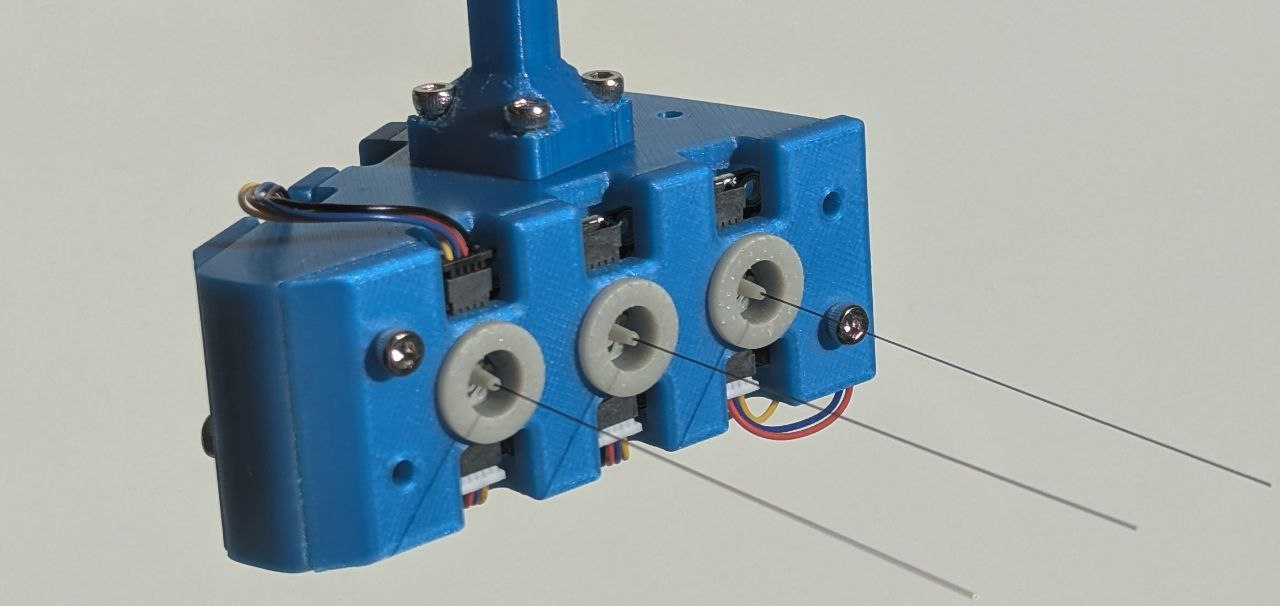
\includegraphics[width=\textwidth]{figures/platform}
    \caption{Assembled whisker platform with three whiskers and robotic arm mount.}
    \label{fig:whisker_platform}
\end{figure}


\section{Data Acquisition}

The Adafruit MLX90393 development board depicted on Figure~\ref{fig:sensor}, which hosts a Hall sensor, is placed approximately \qtyrange{2}{3}{\milli\metre} beneath the suspension-mounted magnet.
The sensor utilizes a 16-bit Analog-to-Digital Converter (ADC) providing magnetic flux density measurements along $X$, $Y$, and $Z$ axes.
It is configured to measure with a resolution of \SI{0.15}{\mu\tesla}.
In practice, only the Y-axis component is used, as it uniquely captures rotation caused by planar whisker deflections.
The sensors communicate via the I2C protocol, operating in slave mode.
When multiple sensors are used, they are connected in a daisy-chain arrangement.

Two drivers have been developed for the MLX90393 sensors: one in C++ for the ESP32 microcontroller and another in Python for the Raspberry Pi 5.
Both implementations follow the official MLX90393 Triaxis Magnetic Node specification~\cite{MLX90393}.
Continuous burst mode is employed, reading sensor data at regular intervals, allowing a data acquisition rate of \SI{300}{\hertz}.
This high rate facilitates effective signal filtering, especially during rapid whisker movements.
The control loop itself operates at approximately \SI{30}{\hertz}, constrained by the actuator’s responsiveness.

\begin{figure}[ht]
    \centering
    \begin{subfigure}[b]{0.45\textwidth}
        \centering
        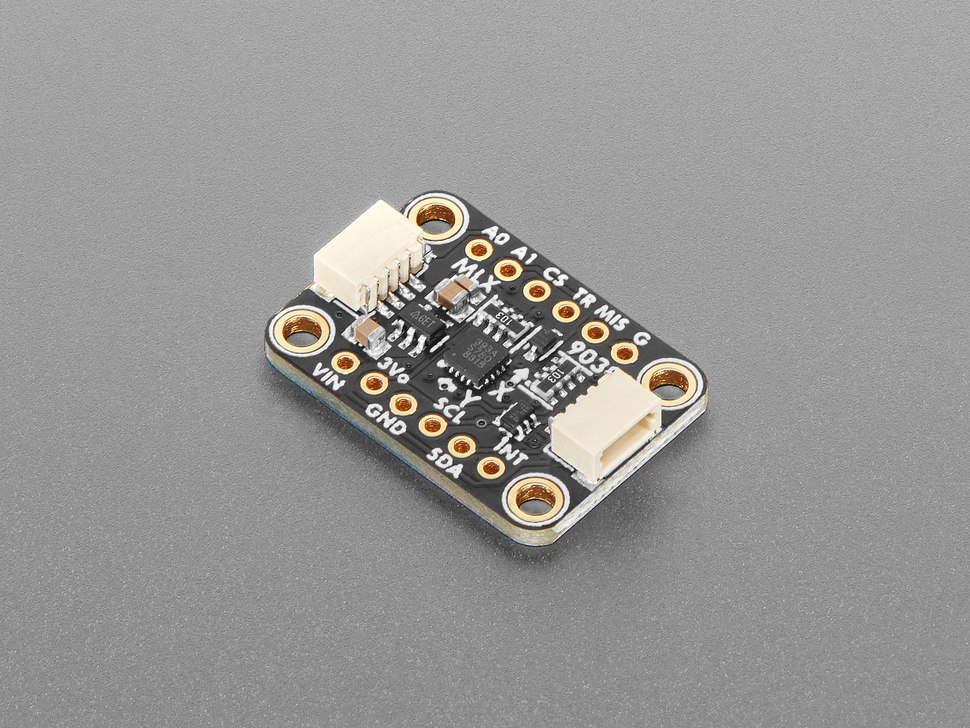
\includegraphics[width=\linewidth]{figures/mlx90393}
        \caption{Adafruit MLX90393 devboard (\SI{25.4}{\milli\meter} $\times$ \SI{17.8}{\milli\meter} $\times$ \SI{1.6}{\milli\meter})}
    \end{subfigure}
    \hfill
    \begin{subfigure}[b]{0.45\textwidth}
        \centering
        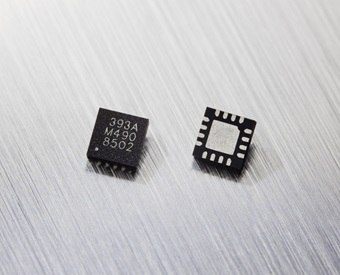
\includegraphics[width=\linewidth]{figures/mlx90393-chip}
        \caption{Melexis MLX90393 chip (\SI{3.1}{\milli\meter} $\times$ \SI{2.9}{\milli\meter} $\times$ \SI{1}{\milli\meter})}
    \end{subfigure}
    \caption{MLX90393 sensor hardware from \cite{MLX90393}}
    \label{fig:sensor}
\end{figure}

The deflection model from the work of \textcite{dang2025whisker} is used to convert the sensor readings into whisker deflection angles.
The model characterizes the deflection profile using two key components: the root position, denoted as \(p_r\), and a measurement model that maps the tangential contact location \(c_t = (x_{bt}, y_{tb})\) (expressed in the sensor base frame) to a deflection measurement \(z\).
In this setup, the bending of the whisker shaft is proportional to the rotation of its suspension system, and the sensor extracts the flux change along the Y-axis—where the variation is most significant—to represent \(z\).

To calibrate this model, the sensor is mounted on a two-dimensional motorized stage, which moves in 3\,mm steps along both axes.
A total of 180 data sets are collected by recording both the magnetic sensor data and the tangential contact positions as the stage moves in a grid-like pattern.
These data are then used to fit a fifth-order bivariate polynomial, yielding a function \(z_c = f(x_b, y_b)\) that describes the deflection arc shape at a given moment.
Note that the default root position is set as \(p_r = (0,0)\), even though slight linear displacements at the center of rotation may occur due to the current spring design—a factor identified for future improvement.

In practice, the provided model covers the operational deflection range (\qtyrange{-5e-5}{5e-4}{\radian}) and starts to diverge from the actual deflection profile at larger angles.
To rectify this, the polynomial is stabilized by clipping values that exceed realistic deflection limits.
Figure~\ref{fig:deflection_profile} illustrates this tweaked deflection profile.

\begin{figure}[htb]
    \centering
    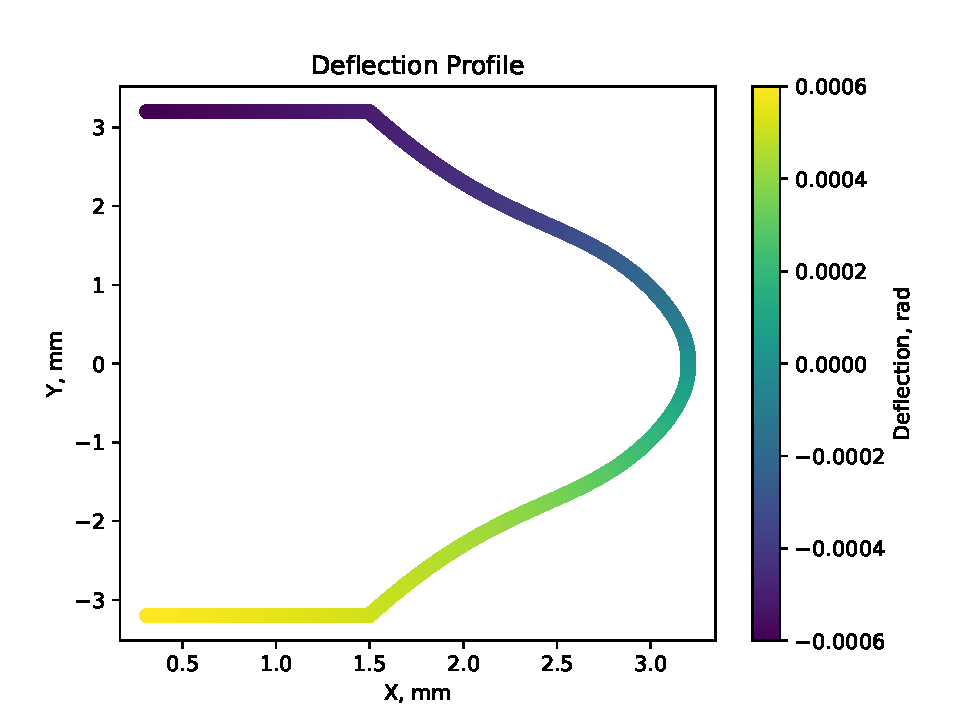
\includegraphics[width=0.8\textwidth]{figures/deflection_profile}
    \caption{Whisker deflection profile model.}
    \label{fig:deflection_profile}
\end{figure}
